\label{section:rel-supervised}
\section{Supervised approaches} 
Supervised methods rely on datasets with human-labeled ground-truth annotations. For example, the SumMe dataset \cite{SumMe} utilizes video summaries as ground truth, while the TVSum dataset \cite{TVSum} employs frame-level importance scores. By leveraging this labeled data, supervised approaches aim to learn the criteria for selecting video frames or fragments to construct effective video summaries.

\subsection{Supervision on frame importance with inter-frame temporal dependency}
\label{subsec:rel-sup-temporal-dependency}

Early deep-learning-based approaches for video summarization treat the task as a structured prediction problem, aiming to estimate the importance of video frames by modeling their temporal dependencies. During the training phase, these approaches utilize ground-truth data indicating frame importance based on user preferences (see \hyperref[figure:rel-sup-model]{Figure \ref{figure:rel-sup-model}}). The frames' temporal dependencies are modeled, and importance scores are predicted, which are then compared with the ground-truth data to guide the training of the summarization model.

\begin{figure}[ht]
  \centering
  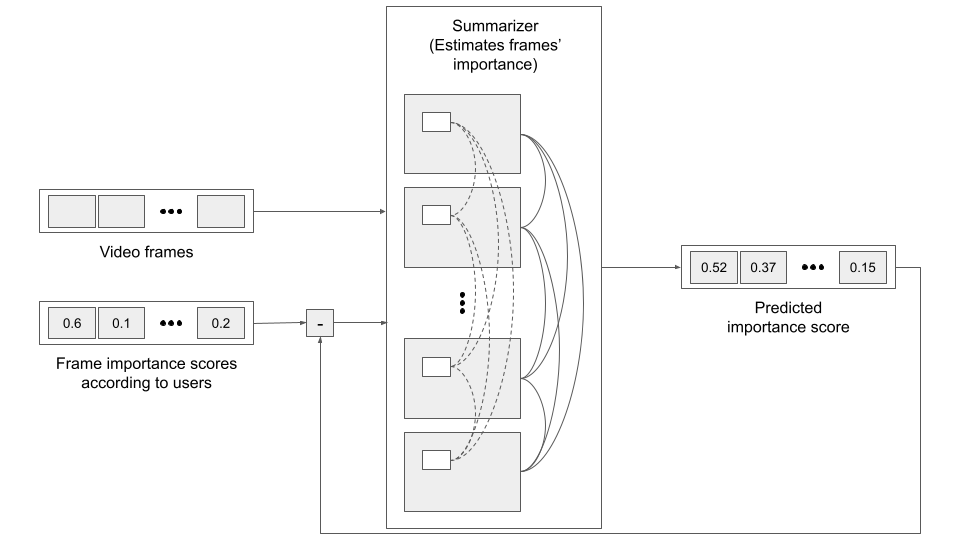
\includegraphics[width=0.73\paperwidth]{content/related/figures/sup-model.png}
  \caption{ High-level representation of the analysis pipeline of supervised algorithms that perform summarization by learning the frames' importance after modeling their temporal or spatiotemporal dependency. For the latter class of methods (i.e., modeling the spatiotemporal dependency among frames), object bounding boxes and object relations in time shown with dashed rectangles and lines, are used to illustrate the extension that models both the temporal and spatial dependency among frames.}
  \label{figure:rel-sup-model}
\end{figure}

One of the initial approaches by Zhang \etal~\cite{zhang2016lstm} employed Long Short-Term Memory (LSTM) units to model variable-range temporal dependencies among video frames. Frame importance was estimated using a multi-layer perceptron (MLP), and diversity in the generated summary's visual content was enhanced using Determinantal Point Process (DPP). Zhao \etal~\cite{zhao2017hierarchical} introduced a two-layer LSTM architecture. The first layer extracted and encoded video structure data, while the second layer estimated fragment-level importance and selected key fragments. In their subsequent work, Zhao \etal~\cite{zhao2018hsa} incorporated a component that learned to identify shot-level temporal structure, enabling importance estimation at the shot level and producing a key-shot-based video summary. Extending their method, Zhao \etal~\cite{zhao2020tth} introduced a tensor-train embedding layer to address large feature-to-hidden mapping matrices. This layer, combined with a hierarchical structure of recurrent neural networks (RNNs), captured temporal dependencies within manually-defined video subshots and across different subshots, determining the probability of each subshot being selected for the video summary.

Lebron Casas \etal~\cite{lebron2019attention} expanded on the work of Zhang \etal~\cite{zhang2016lstm} by incorporating an attention mechanism to model the temporal evolution of users' interest. This information was then used to estimate frame importance and select keyframes for constructing a video storyboard. Several other methods adopted sequence-to-sequence (seq2seq) architectures with attention mechanisms. Ji \etal~\cite{ji2019attentionEnDe} formulated video summarization as a seq2seq learning problem, using an LSTM-based encoder-decoder network with an intermediate attention layer. They extended their model in Ji \etal~\cite{ji2020deep} by integrating a semantic preserving embedding network and employing the Huber loss instead of Mean Square Error (MSE) loss for enhanced robustness. Fajtl \etal~\cite{fajtl2019summarizing} utilized a soft self-attention mechanism and a two-layer fully connected network for regression to estimate frame importance, avoiding computationally-demanding LSTMs. Liu \etal~\cite{liu2019learning} proposed a hierarchical approach combining a generator-discriminator architecture to estimate shot representativeness and select candidate keyframes, followed by a multi-head attention model for further importance assessment and final keyframe selection. Li \etal~\cite{li2021exploring} introduced a global diverse attention mechanism based on the self-attention mechanism of the Transformer Network, encoding temporal relations between frames and transforming diverse attention weights into importance scores.

Another approach, presented by Rochan \etal~\cite{rochan2018sequence}, treated video summarization as a semantic segmentation task, treating the video as a 1D image and employing semantic segmentation models such as Fully Convolutional Networks (FCN) and DeepLab. They developed a network called Fully Convolutional Sequence Network that effectively modeled long-range dependencies among frames and learned frame importance by using convolutions with increasing effective context size.

To address the limited capacity of LSTMs, some techniques incorporated additional memory. Feng \etal~\cite{feng2018memory} proposed a deep learning architecture that stored information about the entire video in an external memory, allowing each shot's importance to be predicted by learning an embedding space for matching shots with the memory information. Wang \etal~\cite{wang2019stacked} stacked multiple LSTM and memory layers hierarchically to capture long-term temporal context and estimate frame importance based on this information.


\subsection{Supervision on frame importance with video spatiotemporal structure}
\label{subsec:rel-sup-spatiotemporal}

% In order to improve the estimation of video frame/fragment importance, certain techniques focus on capturing both the spatial and temporal structure of the video. These approaches not only take into account the input sequence of video frames and the available ground-truth data indicating frame importance, but also model the spatiotemporal dependencies among frames. This additional analysis enhances the training process of the Summarizer, as shown by the dashed rectangles and lines in Figure 3.

% Lal et al. (2019) introduced an encoder-decoder architecture with convolutional LSTMs that effectively models the spatiotemporal relationships within the video. The algorithm not only estimates frame importance but also enhances visual diversity through next frame prediction and shot detection mechanisms, leveraging the likelihood that initial frames of a shot are often part of the summary.

% Yuan et al. (2019) employed a trainable 3D-CNN to extract deep and shallow features from the video content and fused them to create a new representation. This representation, combined with convolutional LSTMs, captures the spatial and temporal structure of the video. A novel loss function called Sobolev loss is then used to learn summarization by minimizing the distance between the series of frame-level importance scores and the ground-truth scores, effectively exploiting the temporal structure of the video.

% Chu et al. (2019) leveraged CNNs to extract spatial and temporal information from raw frames and optical flow maps. Through a label distribution learning process, they learned to estimate frame importance based on human annotations. 

% Elfeki et al. (2019) combined CNNs and Gated Recurrent Units (GRUs), a type of RNN, to form spatiotemporal feature vectors. These vectors were used to estimate the level of activity and importance for each frame.

% Huang et al. (2020) trained a neural network to extract spatiotemporal information from the video, specifically focusing on inter-frame motion. This information was used to create an inter-frames motion curve, which was then input into a transition effects detection method for shot segmentation. A self-attention model, guided by human-generated ground-truth data, was employed to estimate intra-shot importance and select key frames/fragments for creating static/dynamic video summaries.

% By incorporating the spatial and temporal aspects of videos, these supervised approaches improve the accuracy of frame importance estimation and enable the generation of more informative video summaries.

\subsection{Supervision on summary authenticity with discriminative adversarial learning}
\label{subsec:rel-sup-discriminative}

% Taking a distinct approach to bridge the gap between machine-generated and ground-truth summaries, certain methods leverage Generative Adversarial Networks (GANs). Illustrated in Figure 4, the Summarizer, acting as the GAN's Generator, takes the video frames as input and generates a summary by computing frame-level importance scores. These predicted scores, along with an optimal video summary based on user preferences, are fed to a trainable Discriminator, which evaluates their similarity and outputs a corresponding score. The training process encompasses an adversarial framework where the Summarizer aims to deceive the Discriminator by producing summaries that are indistinguishable from the user-generated ones, while the Discriminator learns to differentiate between them. When the Discriminator's confidence level becomes low, indicating an equal classification error for both machine- and user-generated summaries, the Summarizer successfully generates summaries that align closely with users' expectations. Zhang et al. (2019) introduced a method that employs LSTMs and Dilated Temporal Relational (DTR) units to capture temporal dependencies across different time windows. Their approach trains the Summarizer by attempting to mislead a trainable discriminator into distinguishing between machine-generated summaries, ground-truth summaries, and randomly created summaries. Fu et al. (2019) proposed an adversarial learning technique for (semi-)supervised video summarization, where the Generator/Summarizer is an attention-based Pointer Network. It determines the start and end points of each video fragment used in the summary. The Discriminator, a 3D-CNN classifier, determines whether a fragment belongs to a ground-truth or machine-generated summary. Instead of using a conventional adversarial loss, their algorithm employs the output of the Discriminator as a reward for training the Generator/Summarizer through reinforcement learning. While the use of GANs in supervised video summarization is relatively limited, this machine learning framework has been extensively employed in unsupervised video summarization, which will be discussed in the subsequent section.
